%package list
%%%%%%%%%%%%%%%%%%%%%%%%%%%%%%%%%%%%%%%%%%%%%%%%%%
\documentclass{article}
\usepackage[top=3cm, bottom=3cm, outer=3cm, inner=3cm]{geometry}
\usepackage{multicol}
\usepackage{graphicx}                  %LINE 225 C1 Y C2
\usepackage{url}
%\usepackage{cite}
\usepackage{hyperref}
\usepackage{array}
%\usepackage{multicol}
\newcolumntype{x}[1]{>{\centering\arraybackslash\hspace{0pt}}p{#1}}
\usepackage{natbib}
\usepackage{pdfpages}
\usepackage{multirow}
\usepackage[normalem]{ulem}
\useunder{\uline}{\ul}{}
\usepackage{svg}
\usepackage{xcolor}
\usepackage{listings}
\lstdefinestyle{ascii-tree}{
    literate={├}{|}1 {─}{--}1 {└}{+}1 
  }
\lstset{basicstyle=\ttfamily,
  showstringspaces=false,
  commentstyle=\color{red},
  keywordstyle=\color{blue}
}
%\usepackage{booktabs}
\usepackage{caption}
\usepackage{subcaption}
\usepackage{float}
\usepackage{array}

\newcolumntype{M}[1]{>{\centering\arraybackslash}m{#1}}
\newcolumntype{N}{@{}m{0pt}@{}}


%%%%%%%%%%%%%%%%%%%%%%%%%%%%%%%%%%%%%%%%%%%%%%%%%%%%%%%%%%%%%%%%%%%%%%%%%%%%
%%%%%%%%%%%%%%%%%%%%%%%%%%%%%%%%%%%%%%%%%%%%%%%%%%%%%%%%%%%%%%%%%%%%%%%%%%%%
\newcommand{\itemEmail}{aquispearr@unsa.edu.pe}

\newcommand{\itemStudentB}{Quispe Arratea Alexandra Raquel}   
\newcommand{\itemStudentB}{Arias Quispe Jhonathan David}   %line 134
%line 134

\newcommand{\itemCourse}{FP-II}
\newcommand{\itemCourseCode}{20212722}
\newcommand{\itemSemester}{II}
\newcommand{\itemUniversity}{Universidad Nacional de San Agustín de Arequipa}
\newcommand{\itemFaculty}{Facultad de Ingeniería de Producción y Servicios}
\newcommand{\itemDepartment}{Departamento Académico de Ingeniería de Sistemas e Informática}
\newcommand{\itemSchool}{Escuela Profesional de Ingeniería de Sistemas}
\newcommand{\itemAcademic}{2023 - B}
\newcommand{\itemInput}{Del 15 Enero 2024}
\newcommand{\itemOutput}{Al 2 Febrero 2024}
\newcommand{\itemPracticeNumber}{24}

%%%%%%%%%%%%%%%%%%%%%%%%%%%%%%%%%%%%%%%%%%%%%%%%%%%%%%%%%%%%%%%%%%%%%%%%%%%%
%%%%%%%%%%%%%%%%%%%%%%%%%%%%%%%%%%%%%%%%%%%%%%%%%%%%%%%%%%%%%%%%%%%%%%%%%%%%

\usepackage[english,spanish]{babel}
\usepackage[utf8]{inputenc}
\AtBeginDocument{\selectlanguage{spanish}}
\renewcommand{\figurename}{Figura}
\renewcommand{\refname}{Referencias}
\renewcommand{\tablename}{Tabla} %esto no funciona cuando se usa babel
\AtBeginDocument{%
	\renewcommand\tablename{Tabla}
}

\usepackage{fancyhdr}
\pagestyle{fancy}
\fancyhf{}
\setlength{\headheight}{30pt}
\renewcommand{\headrulewidth}{1pt}
\renewcommand{\footrulewidth}{1pt}
\fancyhead[L]{\raisebox{-0.2\height}{
\includegraphics[width=3cm]{img/logo_episunsa.png}}}
\fancyhead[C]{\fontsize{7}{7}\selectfont	\itemUniversity \\ \itemFaculty \\ \itemDepartment \\ \itemSchool \\ \textbf{\itemCourse}}
\fancyhead[R]{\raisebox{-0.2\height}{
\includegraphics[width=1.2cm]{img/logo_abet}}}
\fancyfoot[L]{Quispe Alexandra - Arias Jhonatan}
\fancyfoot[C]{\itemCourse}
\fancyfoot[R]{Página \thepage}

% para el codigo fuente
\usepackage{listings}
\usepackage{color, colortbl}
\definecolor{dkgreen}{rgb}{0,0.6,0}
\definecolor{gray}{rgb}{0.5,0.5,0.5}
\definecolor{mauve}{rgb}{0.58,0,0.82}
\definecolor{codebackground}{rgb}{0.95, 0.95, 0.92}
\definecolor{tablebackground}{rgb}{0.8, 0, 0}

\lstset{frame=tb,
	language=bash,
	aboveskip=3mm,
	belowskip=3mm,
	showstringspaces=false,
	columns=flexible,
	basicstyle={\small\ttfamily},
	numbers=none,
	numberstyle=\tiny\color{gray},
	keywordstyle=\color{blue},
	commentstyle=\color{dkgreen},
	stringstyle=\color{mauve},
	breaklines=true,
	breakatwhitespace=true,
	tabsize=3,
	backgroundcolor= \color{codebackground},
}

\begin{document}
	
	\vspace*{10px}
	
	\begin{center}	
		\fontsize{17}{17} \textbf{Informe de Laboratorio Final \itemPracticeNumber}
	\end{center}

	\begin{flushright}
		\begin{tabular}{|M{2.5cm}|N|}
			\hline 
			\rowcolor{tablebackground}
			\color{white} \textbf{Nota}  \\
			\hline 
			     \\[30pt]
			\hline 			
		\end{tabular}
	\end{flushright}	

	\begin{table}[H]
		\begin{tabular}{|x{4.7cm}|x{4.8cm}|x{4.8cm}|}
			\hline                                       %line 41
			\rowcolor{tablebackground}
			\color{white} \textbf{Estudiante} & \color{white}\textbf{Escuela}  & \color{white}\textbf{Asignatura}   \\
			\hline 
			{ \itemStudentA \par \itemStudentB \par \itemStudentC \par \itemStudentD \par\itemStudentE} &
			\itemSchool & {\itemCourse \par Semestre: \itemSemester}     \\
			\hline 			
		\end{tabular}
	\end{table}		
	
	\begin{table}[H]
		\begin{tabular}{|x{4.7cm}|x{4.8cm}|x{4.8cm}|}
			\hline 
			\rowcolor{tablebackground}
			\color{white}\textbf{Laboratorio} & \color{white}\textbf{Tema}  & \color{white}\textbf{Duración}   \\
			\hline 
			\itemPracticeNumber & \itemTheme & 24 horas aprox.\\
			\hline 
		\end{tabular}
	\end{table}
	
	\begin{table}[H]
		\begin{tabular}{|x{4.7cm}|x{4.8cm}|x{4.8cm}|}
			\hline 
			\rowcolor{tablebackground}
			\color{white}\textbf{Semestre académico} & \color{white}\textbf{Fecha de inicio}  & \color{white}\textbf{Fecha de entrega}   \\
			\hline 
			\itemAcademic & \itemInput &  \itemOutput  \\
			\hline 
		\end{tabular}
	\end{table}
	
	\section{Tarea}
	\begin{itemize}		%line 200 first commit
		\item \textbf{}
Cree una versión del videojuego de estrategia usando componentes básicos GUI: Etiquetas, botones,
cuadros de texto, JOptionPane, Color.
Además, utilizar componentes avanzados GUI: Layouts, JPanel, áreas de texto, checkbox, botones de
radio y combobox.
Considerar nivel estratégico y táctico.
Considerar hasta las unidades especiales de los reinos.
Hacerlo iterativo.
 

	\end{itemize}
		
	\section{Equipos, materiales y temas utilizados}
	\begin{itemize}
		\item Sistemas Operativos Ubuntu y Windows 
		\item NVIM v0.6.1, VSCode, Eclipse
		\item OpenJDK 64-Bits 11, 17, 18
		\item Git 2.34.1 y versiones posteriores
		\item Cuentas en GitHub con el correo institucional.
		\item Programación Orientada a Objetos.
		\item Algoritmos de ordenamiento y búsqueda
		\item Modelizado de algoritmos
	\end{itemize}
	
	\section{URL de Repositorio Github}
	\begin{itemize}
		\item URL del Repositorio GitHub para clonar o recuperar.
		\item \url{https://github.com/JhonatanDczel/FP2-trabajo-final.git}
	\end{itemize}
	
	

%%%%%%%%%%%%%%%%%%%%%%%%%%%%%%%%%%%%%%%%%%%%%%%%%%%%%%%%%%%%%%%%%%%%%%%%%%%%%%%%%%%%%%%%%%%%%%%%%%%%%%%%%%%%%%%%%%%%%%%%%%%%%%%%%%%%%%%%%%%%%%%%%%%%%%%%%%%%%%%%%%%%%%%%%%%%%%%%%%%%%%%%%%%%%%%%%%%
\section{Proyecto LabFinal}
 

            \begin{itemize}
                \item Generamos diagrama UML del proyecto :
            \end{itemize}
            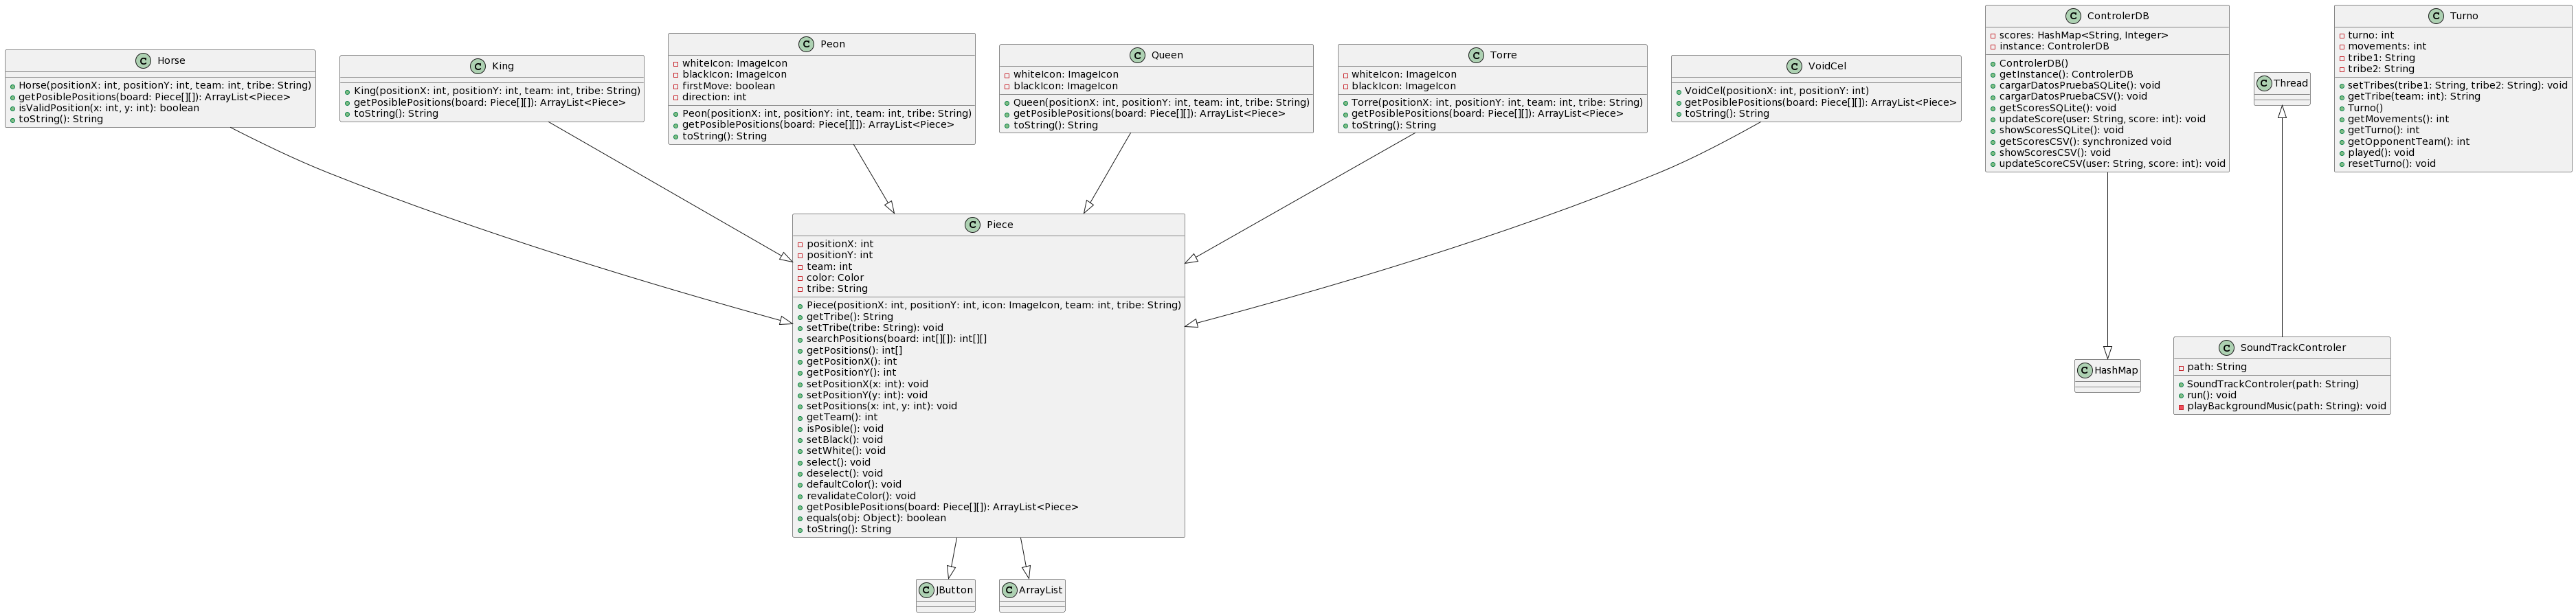
\includegraphics[width=18cm]{latex/img/uml.png}
\section{Contextualización del Juego}

En este proyecto, hemos tomado la base de un juego de estrategia con soldados y lo hemos adaptado para crear un emocionante juego de ajedrez con funciones más dinámicas. Esta adaptación sigue aplicando los conceptos aprendidos durante el curso y busca proporcionar a los jugadores una experiencia única en el mundo del ajedrez.

Hemos transformado el juego original para que sea un enfrentamiento uno contra uno, donde los jugadores se dividen en cuatro pueblos, cada uno con características especiales, bonificaciones y penalizaciones. A continuación, presentamos cada uno de los pueblos , detallando sus características únicas.

\subsection{Macondo}
Macondo es un pueblo mágico y aislado, donde ocurren sucesos fantásticos e insólitos. Sus habitantes son soñadores, curiosos y creativos, pero también sufren de olvido. Las fichas de ajedrez podrían tienen un distintivo de un gorro de mago.

\textbf{Bonificación de Portal Mágico:}
Puede intercambiar de lugar dos fichas aliadas una vez por partida.

\textbf{Penalización de Olvido:}
Si Macondo no utiliza su bonificación de portal mágico antes de alcanzar la mitad de la partida, pierde 5 puntos de vida por haber olvidado sus habilidades mágicas.
\begin{center}
    
\includegraphics[width=6cm]{latex/img/Macondo.png}
\end{center}
\subsection{Comala}
Comala es un pueblo fantasmal y desolado, donde los muertos conviven con los vivos. Sus habitantes son silenciosos, melancólicos y resignados, pero también buscan la redención y el perdón. Las fichas de ajedrez podrían tienen un distintivo de una vela, que simboliza la fe y el sufrimiento.

\textbf{Bonificación de Fantasma:}
Puede esquivar un ataque enemigo, reduciendo el daño recibido a la mitad, una vez por turno.

\textbf{Penalización de Soledad:}
Pierde 15 puntos de vida si está completamente rodeado por fichas enemigas.
\begin{center}
    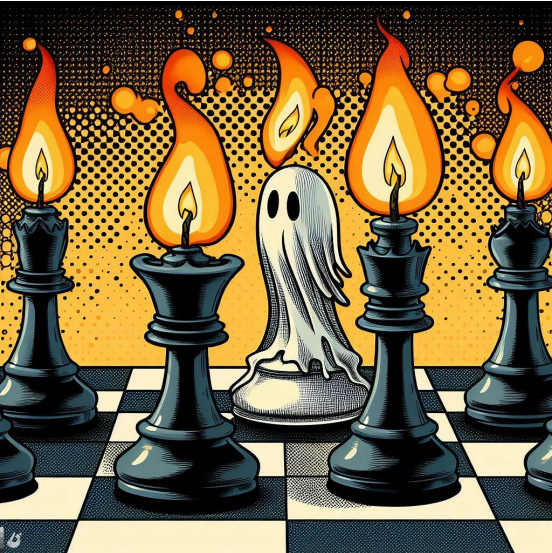
\includegraphics[width=6cm]{latex/img/Comala.png}
\end{center}
\subsection{Rivendel}
Rivendel es un reino élfico y hermoso, donde reina la armonía y la sabiduría. Sus habitantes son ágiles, bellos y sabios, pero también nostálgicos y orgullosos. Las fichas de ajedrez podrían tener un distintivo de una corona de oro, que simboliza la luz y la elegancia.

\textbf{Bonificación de Luz Élfica:}
Puede realizar un movimiento especial (moverse donde sea) una vez por partida que afecta a una ficha enemiga cercana.

\textbf{Penalización de Nostalgia:}
La añoranza de Rivendel lo distrae, perdiendo 20 puntos de ataque si se aleja más de tres casillas de su posición inicial.
\begin{center}
    \includegraphics[width=6cm]{latex/img/RIvendel.png}
\end{center}
\subsection{Dorne}
Dorne es un reino sureño y exótico, donde se celebra la diversidad y la libertad. Sus habitantes son carismáticos, seductores y venenosos, pero también rebeldes e indomables. Las fichas de ajedrez podrían tener un distintivo de tatuajes, que simboliza el exotismo.

\textbf{Bonificación de Solidaridad Exótica:}
Puede transferir 10 puntos de defensa adicional a una ficha aliada una vez por turno.

\textbf{Penalización de Rebeldía:}
La rebeldía de Dorne aumenta su fuerza, pero también su vulnerabilidad. Obtendrá un bonus de ataque aleatorio (entre 10 y 30 puntos), pero perderá 15 puntos de defensa.
\begin{center}
    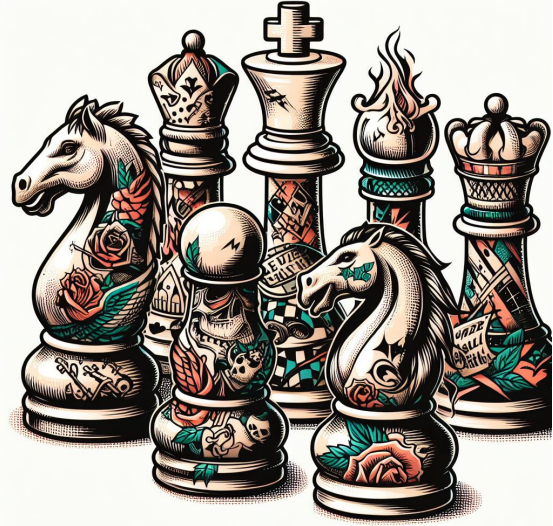
\includegraphics[width=6cm]{latex/img/Dorne.png}
\end{center}

\section{Desarrollo de clases}

\subsection{Clase BattleWindow}
La clase \texttt{BattleWindow} representa la ventana de la batalla en el juego. A continuación, se presenta un resumen de su estructura y funcionamiento:

\subsubsection{Atributos:}
\begin{itemize}
  \item \texttt{attacker}: Pieza atacante en la batalla.
  \begin{lstlisting}[language=java,caption={Atributo \texttt{attacker} en la clase \texttt{BattleWindow}}]
    private Piece attacker;
  \end{lstlisting}

  \item \texttt{defender}: Pieza defensora en la batalla.
  \begin{lstlisting}[language=java,caption={Atributo \texttt{defender} en la clase \texttt{BattleWindow}}]
    private Piece defender;
  \end{lstlisting}
\end{itemize}

\subsubsection{Métodos Relevantes:}
\begin{itemize}
  \item \texttt{BattleWindow(Piece attacker, Piece defender)}: Constructor que inicializa la ventana de la batalla con las piezas proporcionadas.
  \begin{lstlisting}[language=java,caption={Constructor \texttt{BattleWindow} que recibe las piezas atacante y defensora}]
    public BattleWindow(Piece attacker, Piece defender) {
      this.attacker = attacker;
      this.defender = defender;

      // Configuración de la interfaz gráfica y creación de paneles
      // ...

      // Agrega las imágenes a los paneles
      attackerPanel.add(attackerLabel);
      defenderPanel.add(defenderLabel);

      // Configuración y visualización de la ventana
      setSize(300, 300);
      setLocationRelativeTo(null);
      setDefaultCloseOperation(JFrame.DISPOSE_ON_CLOSE);
      setVisible(true);
    }
  \end{lstlisting}

  \item \texttt{BattleBar}: Clase interna que representa la barra de la batalla y calcula el resultado de la misma.
  \begin{lstlisting}[language=java,caption={Clase interna \texttt{BattleBar} en la clase \texttt{BattleWindow}}]
    private class BattleBar extends JPanel {
      // Implementación de la clase interna
      // ...
    }
  \end{lstlisting}

  \item \texttt{calculateBattleResult()}: Método que debe ser implementado para calcular el resultado de la batalla. Retorna un valor entre 0 y 100 representando el porcentaje de éxito del atacante.
  \begin{lstlisting}[language=java,caption={Método \texttt{calculateBattleResult} en la clase \texttt{BattleBar}}]
    private int calculateBattleResult() {
      // Método que debes implementar para calcular el resultado de la batalla
      // Debes retornar un valor entre 0 y 100 representando el porcentaje de éxito del atacante
      return 50; // Ejemplo: Empate
    }
  \end{lstlisting}
\end{itemize}

Esta clase proporciona una interfaz gráfica para visualizar la batalla entre dos piezas en el juego. La barra horizontal en el centro de la ventana representa visualmente el resultado de la batalla.

%%%%%%%%%%%%%%%%%%%%%%%%%%%%%%%%%%%%%%%%%%%%%%%%%%%%%%%%%%%%%%%%%%%%%%%%%%%
\subsection{Clase Board}
La clase \texttt{Board} representa el tablero del juego de ajedrez. A continuación, se presenta un resumen de su estructura y funcionamiento:

\subsubsection{Atributos:}
\begin{itemize}
  \item \texttt{board}: Matriz que representa el tablero de juego.
  \begin{lstlisting}[language=java,caption={Atributo \texttt{board} en la clase \texttt{Board}}]
    private Piece[][] board = new Piece[8][8];
  \end{lstlisting}

  \item \texttt{turno}: Objeto que lleva el control del turno actual.
  \begin{lstlisting}[language=java,caption={Atributo \texttt{turno} en la clase \texttt{Board}}]
    private Turno turno = new Turno();
  \end{lstlisting}

  \item \texttt{finishBtn}: Pieza que representa la posición de inicio del movimiento.
  \begin{lstlisting}[language=java,caption={Atributo \texttt{finishBtn} en la clase \texttt{Board}}]
    private Piece finishBtn = null;
  \end{lstlisting}

  \item \texttt{posiblePositions}: Lista de posiciones posibles para una pieza.
  \begin{lstlisting}[language=java,caption={Atributo \texttt{posiblePositions} en la clase \texttt{Board}}]
    private ArrayList<Piece> posiblePositions;
  \end{lstlisting}

  \item \texttt{box1, box2}: Paneles que contienen componentes del juego.
  \begin{lstlisting}[language=java,caption={Atributos \texttt{box1} y \texttt{box2} en la clase \texttt{Board}}]
    private JPanel box1;
    private JPanel box2;
  \end{lstlisting}

  \item \texttt{btnSave, btnRecover, btnNewPLay}: Botones para guardar, recuperar y reiniciar el juego.
  \begin{lstlisting}[language=java,caption={Atributos \texttt{btnSave}, \texttt{btnRecover}, y \texttt{btnNewPLay} en la clase \texttt{Board}}]
    private JButton btnSave = new JButton("SAVE GAME");
    private JButton btnRecover = new JButton("RECOVER GAME");
    private JButton btnNewPLay = new JButton("NEW PLAY");
  \end{lstlisting}
\end{itemize}

\subsubsection{Métodos Relevantes:}
\begin{itemize}
  \item \texttt{Board()}: Constructor que inicia un nuevo juego de ajedrez.
  \begin{lstlisting}[language=java,caption={Constructor \texttt{Board} en la clase \texttt{Board}}]
    public Board() {
      // Implementación del constructor
      // ...
    }
  \end{lstlisting}

  \item \texttt{ListenerBtn}: Clase interna que implementa \texttt{ActionListener} para manejar eventos de botones.
  \begin{lstlisting}[language=java,caption={Clase interna \texttt{ListenerBtn} en la clase \texttt{Board}}]
    private class ListenerBtn implements ActionListener {
      // Implementación de la clase interna
      // ...
    }
  \end{lstlisting}

  \item \texttt{resetGame()}: Reinicia el juego con nuevas tribus.
  \begin{lstlisting}[language=java,caption={Método \texttt{resetGame} en la clase \texttt{Board}}]
    public void resetGame() {
      // Implementación del reinicio del juego
      // ...
    }
  \end{lstlisting}

  \item \texttt{saveGame()}: Guarda el estado actual del juego en un archivo binario.
  \begin{lstlisting}[language=java,caption={Método \texttt{saveGame} en la clase \texttt{Board}}]
    public void saveGame() {
      // Implementación del guardado del juego
      // ...
    }
  \end{lstlisting}

  \item \texttt{recoverGame()}: Recupera un juego guardado anteriormente.
  \begin{lstlisting}[language=java,caption={Método \texttt{recoverGame} en la clase \texttt{Board}}]
    public void recoverGame() {
      // Implementación de la recuperación del juego
      // ...
    }
  \end{lstlisting}

  \item \texttt{removeBoard()}: Elimina las piezas del tablero.
  \begin{lstlisting}[language=java,caption={Método \texttt{removeBoard} en la clase \texttt{Board}}]
    public void removeBoard() {
      // Implementación de la eliminación de las piezas del tablero
      // ...
    }
  \end{lstlisting}

  \item \texttt{reFill()}: Vuelve a llenar el tablero con las piezas.
  \begin{lstlisting}[language=java,caption={Método \texttt{reFill} en la clase \texttt{Board}}]
    public void reFill() {
      // Implementación del rellenado del tablero
      // ...
    }
  \end{lstlisting}
\end{itemize}

La clase \texttt{Board} proporciona la lógica y la interfaz para el juego de ajedrez, gestionando el tablero, las piezas y las interacciones entre los jugadores.


&&&&&&&&&&&&&&&&&&&&&&&&&&&&&&&&&&&&&&&&&&&&&&&&&&&&&&&&&&&&&&&&&&&&&&&&&&&&&
\subsection{Clase Horse}
La clase \texttt{Horse} representa la pieza de caballo en el juego de ajedrez. A continuación, se presenta un resumen de su estructura y funcionamiento:

\subsubsection{Atributos:}
\begin{itemize}
  \item \texttt{whiteIcon, blackIcon}: Iconos para la pieza de caballo en los equipos blanco y negro.
  \begin{lstlisting}[language=java,caption={Atributos \texttt{whiteIcon} y \texttt{blackIcon} en la clase \texttt{Horse}}]
    private static ImageIcon whiteIcon = new ImageIcon("./assets/whiteHorse.png");
    private static ImageIcon blackIcon = new ImageIcon("./assets/blackHorse.png");
  \end{lstlisting}
\end{itemize}

\subsubsection{Métodos Relevantes:}
\begin{itemize}
  \item \texttt{Horse(int positionX, int positionY, int team, String tribe)}: Constructor que inicializa la pieza de caballo con la posición, equipo y tribu correspondientes.
  \begin{lstlisting}[language=java,caption={Constructor \texttt{Horse} en la clase \texttt{Horse}}]
    public Horse(int positionX, int positionY, int team, String tribe) {
      // Implementación del constructor
      // ...
    }
  \end{lstlisting}

  \item \texttt{getPosiblePositions(Piece[][] board)}: Obtiene las posiciones posibles a las que puede moverse la pieza de caballo.
  \begin{lstlisting}[language=java,caption={Método \texttt{getPosiblePositions} en la clase \texttt{Horse}}]
    public ArrayList<Piece> getPosiblePositions(Piece[][] board) {
      // Implementación del método
      // ...
    }
  \end{lstlisting}

  \item \texttt{isValidPosition(int x, int y)}: Verifica si una posición dada en el tablero es válida.
  \begin{lstlisting}[language=java,caption={Método \texttt{isValidPosition} en la clase \texttt{Horse}}]
    private boolean isValidPosition(int x, int y) {
      // Implementación del método
      // ...
    }
  \end{lstlisting}

  \item \texttt{toString()}: Devuelve una representación en cadena de la pieza de caballo.
  \begin{lstlisting}[language=java,caption={Método \texttt{toString} en la clase \texttt{Horse}}]
    public String toString(){
      return "Caballo "+super.toString();
    }
  \end{lstlisting}
\end{itemize}

La clase \texttt{Horse} encapsula la lógica específica del caballo en el juego de ajedrez, determinando sus movimientos posibles y proporcionando una representación en cadena para fines de visualización.



\subsection{Clase King}
La clase \texttt{King} representa la pieza de rey en el juego de ajedrez. A continuación, se presenta un resumen de su estructura y funcionamiento:

\subsubsection{Atributos:}
\begin{itemize}
  \item \texttt{whiteIcon, blackIcon}: Iconos para la pieza de rey en los equipos blanco y negro.
  \begin{lstlisting}[language=java,caption={Atributos \texttt{whiteIcon} y \texttt{blackIcon} en la clase \texttt{King}}]
    private static ImageIcon whiteIcon = new ImageIcon("./assets/whiteKing.png");
    private static ImageIcon blackIcon = new ImageIcon("./assets/blackKing.png");
  \end{lstlisting}
\end{itemize}

\subsubsection{Métodos Relevantes:}
\begin{itemize}
  \item \texttt{King(int positionX, int positionY, int team, String tribe)}: Constructor que inicializa la pieza de rey con la posición, equipo y tribu correspondientes.
  \begin{lstlisting}[language=java,caption={Constructor \texttt{King} en la clase \texttt{King}}]
    public King(int positionX, int positionY, int team, String tribe) {
      // Implementación del constructor
      // ...
    }
  \end{lstlisting}

  \item \texttt{getPosiblePositions(Piece[][] board)}: Obtiene las posiciones posibles a las que puede moverse la pieza de rey.
  \begin{lstlisting}[language=java,caption={Método \texttt{getPosiblePositions} en la clase \texttt{King}}]
    public ArrayList<Piece> getPosiblePositions(Piece[][] board) {
      // Implementación del método
      // ...
    }
  \end{lstlisting}

  \item \texttt{toString()}: Devuelve una representación en cadena de la pieza de rey.
  \begin{lstlisting}[language=java,caption={Método \texttt{toString} en la clase \texttt{King}}]
    public String toString(){
      return "Rey "+super.toString();
    }
  \end{lstlisting}
\end{itemize}

La clase \texttt{King} encapsula la lógica específica del rey en el juego de ajedrez, determinando sus movimientos posibles y proporcionando una representación en cadena para fines de visualización.


\subsection{Clase Peon}
La clase \texttt{Peon} representa la pieza de peón en el juego de ajedrez. A continuación, se presenta un resumen de su estructura y funcionamiento:

\subsubsection{Atributos:}
\begin{itemize}
  \item \texttt{whiteIcon, blackIcon}: Iconos para la pieza de peón en los equipos blanco y negro.
  \begin{lstlisting}[language=java,caption={Atributos \texttt{whiteIcon} y \texttt{blackIcon} en la clase \texttt{Peon}}]
    private static ImageIcon whiteIcon = new ImageIcon("./assets/whitePeon.png");
    private static ImageIcon blackIcon = new ImageIcon("./assets/blackPeon.png");
  \end{lstlisting}
  
  \item \texttt{firstMove}: Indica si es el primer movimiento del peón.
  \begin{lstlisting}[language=java,caption={Atributo \texttt{firstMove} en la clase \texttt{Peon}}]
    private boolean firstMove = true;
  \end{lstlisting}

  \item \texttt{direction}: Dirección del movimiento del peón según el equipo.
  \begin{lstlisting}[language=java,caption={Atributo \texttt{direction} en la clase \texttt{Peon}}]
    private int direction;
  \end{lstlisting}
\end{itemize}

\subsubsection{Métodos Relevantes:}
\begin{itemize}
  \item \texttt{Peon(int positionX, int positionY, int team, String tribe)}: Constructor que inicializa la pieza de peón con la posición, equipo y tribu correspondientes.
  \begin{lstlisting}[language=java,caption={Constructor \texttt{Peon} en la clase \texttt{Peon}}]
    public Peon(int positionX, int positionY, int team, String tribe) {
      // Implementación del constructor
      // ...
    }
  \end{lstlisting}

  \item \texttt{getPosiblePositions(Piece[][] board)}: Obtiene las posiciones posibles a las que puede moverse la pieza de peón.
  \begin{lstlisting}[language=java,caption={Método \texttt{getPosiblePositions} en la clase \texttt{Peon}}]
    public ArrayList<Piece> getPosiblePositions(Piece[][] board) {
      // Implementación del método
      // ...
    }
  \end{lstlisting}

  \item \texttt{toString()}: Devuelve una representación en cadena de la pieza de peón.
  \begin{lstlisting}[language=java,caption={Método \texttt{toString} en la clase \texttt{Peon}}]
    public String toString(){
      return "Peon "+super.toString();
    }
  \end{lstlisting}
\end{itemize}

La clase \texttt{Peon} encapsula la lógica específica del peón en el juego de ajedrez, incluyendo su primer movimiento especial y la determinación de sus movimientos posibles.```

%%%%%%%%%%%%%%%%%%%%%%%%%%%%%%%%%%%%%%%%%%%%

\subsection{Clase Queen}
La clase \texttt{Queen} representa la pieza de reina en el juego de ajedrez. A continuación, se presenta un resumen de su estructura y funcionamiento:

\subsubsection{Atributos:}
\begin{itemize}
  \item \texttt{whiteIcon, blackIcon}: Iconos para la pieza de reina en los equipos blanco y negro.
  \begin{lstlisting}[language=java,caption={Atributos \texttt{whiteIcon} y \texttt{blackIcon} en la clase \texttt{Queen}}]
    private static ImageIcon whiteIcon = new ImageIcon("./assets/whiteQueen.png");
    private static ImageIcon blackIcon = new ImageIcon("./assets/blackQueen.png");
  \end{lstlisting}
\end{itemize}

\subsubsection{Métodos Relevantes:}
\begin{itemize}
  \item \texttt{Queen(int positionX, int positionY, int team, String tribe)}: Constructor que inicializa la pieza de reina con la posición, equipo y tribu correspondientes.
  \begin{lstlisting}[language=java,caption={Constructor \texttt{Queen} en la clase \texttt{Queen}}]
    public Queen(int positionX, int positionY, int team, String tribe) {
      // Implementación del constructor
      // ...
    }
  \end{lstlisting}

  \item \texttt{getPosiblePositions(Piece[][] board)}: Obtiene las posiciones posibles a las que puede moverse la pieza de reina.
  \begin{lstlisting}[language=java,caption={Método \texttt{getPosiblePositions} en la clase \texttt{Queen}}]
    public ArrayList<Piece> getPosiblePositions(Piece[][] board) {
      // Implementación del método
      // ...
    }
  \end{lstlisting}

  \item \texttt{toString()}: Devuelve una representación en cadena de la pieza de reina.
  \begin{lstlisting}[language=java,caption={Método \texttt{toString} en la clase \texttt{Queen}}]
    public String toString(){
      return "Reina "+super.toString();
    }
  \end{lstlisting}
\end{itemize}

La clase \texttt{Queen} encapsula la lógica específica de la reina en el juego de ajedrez, incluyendo la determinación de sus movimientos posibles en diferentes direcciones.```


\subsection{Clase Torre}
La clase \texttt{Torre} representa la pieza de torre en el juego de ajedrez. A continuación, se presenta un resumen de su estructura y funcionamiento:

\subsubsection{Atributos:}
\begin{itemize}
  \item \texttt{whiteIcon, blackIcon}: Iconos para la pieza de torre en los equipos blanco y negro.
  \begin{lstlisting}[language=java,caption={Atributos \texttt{whiteIcon} y \texttt{blackIcon} en la clase \texttt{Torre}}]
    private static ImageIcon whiteIcon = new ImageIcon("./assets/whiteTorre.png");
    private static ImageIcon blackIcon = new ImageIcon("./assets/blackTorre.png");
  \end{lstlisting}
\end{itemize}

\subsubsection{Métodos Relevantes:}
\begin{itemize}
  \item \texttt{Torre(int positionX, int positionY, int team, String tribe)}: Constructor que inicializa la pieza de torre con la posición, equipo y tribu correspondientes.
  \begin{lstlisting}[language=java,caption={Constructor \texttt{Torre} en la clase \texttt{Torre}}]
    public Torre(int positionX, int positionY, int team, String tribe) {
      // Implementación del constructor
      // ...
    }
  \end{lstlisting}

  \item \texttt{getPosiblePositions(Piece[][] board)}: Obtiene las posiciones posibles a las que puede moverse la pieza de torre.
  \begin{lstlisting}[language=java,caption={Método \texttt{getPosiblePositions} en la clase \texttt{Torre}}]
    public ArrayList<Piece> getPosiblePositions(Piece[][] board) {
      // Implementación del método
      // ...
    }
  \end{lstlisting}

  \item \texttt{toString()}: Devuelve una representación en cadena de la pieza de torre.
  \begin{lstlisting}[language=java,caption={Método \texttt{toString} en la clase \texttt{Torre}}]
    public String toString(){
      return "Torre "+super.toString();
    }
  \end{lstlisting}
\end{itemize}

La clase \texttt{Torre} encapsula la lógica específica de la torre en el juego de ajedrez, incluyendo la determinación de sus movimientos posibles en direcciones vertical y horizontal.```

\subsection{Clase VoidCel:}
A continuación se presenta el código de la clase que representa una celda vacía en un tablero de ajedrez en Java.

\begin{lstlisting}[language=java,caption={Clase VoidCel}]
import java.awt.Cursor;
import java.util.ArrayList;

public class VoidCel extends Piece {
  public VoidCel(int positionX, int positionY) {
    super(positionX, positionY, null, -1, "none");
    setCursor(new Cursor(Cursor.DEFAULT_CURSOR));
  };

  public ArrayList<Piece> getPosiblePositions(Piece[][] board) {
    return new ArrayList<Piece>();
  };
  public String toString(){
    return "Vacio "+super.toString();
  }
}
\end{lstlisting}

%%%%%%%%%%%%%%%%%%%%%%%%%%%%%%%%%%%%%%%%%%%%%%%%%%%%%%%%%%%%%%
\subsection{Base de Datos}
Código SQL para crear una base de datos con una tabla de usuarios y datos de ejemplo:

\begin{lstlisting}[language=sql]
-- Crear la base de datos
CREATE DATABASE IF NOT EXISTS fp2_23b;

-- Usar la base de datos
USE fp2_23b;

-- Crear la tabla de usuarios
CREATE TABLE IF NOT EXISTS usuarios (
    id INT AUTO_INCREMENT PRIMARY KEY,
    usuario VARCHAR(255) NOT NULL,
    puntuacion INT NOT NULL
);

-- Insertar datos de ejemplo
INSERT INTO usuarios (usuario, puntuacion) VALUES
('Pepito', 10),
('Juanito', 150),
('Reginald', 80);
\end{lstlisting}


%%%%%%%%%%%%%%%%%%%%%%%%
\subsection{Pista de Sonido}
A continuación, se proporciona el código de un controlador de pista de sonido en Java, diseñado para reproducir música en segundo plano mediante el uso de la biblioteca javax.sound.sampled. Este controlador no solo ofrece funcionalidades estándar para la reproducción de sonido, sino que también implementa técnicas de programación paralela para optimizar el rendimiento y aprovechar eficientemente los recursos del sistema.


Para obtener puntos adicionales, hemos abordado este problema soundtrack . En lugar de reproducirlo como fondo, lo hemos implementado para ejecutarse de forma paralela. Esta solución permite que el soundtrack y el juego se desarrollen simultáneamente, evitando que el programa espere a que el soundtrack finalice para concluir la partida.

\subsubsection{Clase SoundTrackControler:}
\begin{lstlisting}[language=java,caption={Clase SoundTrackControler}]
import javax.sound.sampled.*;
import java.io.File;

public class SoundTrackControler extends Thread {
    private String path;

    public SoundTrackControler(String path) {
        this.path = path;
    }

    @Override
    public void run() {
        playBackgroundMusic(path);
    }

    private void playBackgroundMusic(String path) {
        try {
            Clip clip = AudioSystem.getClip();
            AudioInputStream inputStream = AudioSystem.getAudioInputStream(new File(path));
            clip.open(inputStream);
            clip.start();
            clip.loop(Clip.LOOP_CONTINUOUSLY);
        } catch (Exception e) {
            System.out.println("Error: " + e.getMessage());
        }
    }
}
\end{lstlisting}
%%%%%%%%%%%%%%%%%%%%%%%%%%%%%%%%%%%%%%%%%%%%%%%%%%%%%%%%%%%%%%%%%%

 \section{Ejecucion del Juego}
 
             \begin{itemize}
                \item Primero, se presenta un menú con dos opciones: "Juego Personalizado" y "Juego Rápido". En el caso de seleccionar "Juego Personalizado", el sistema redirige al usuario a una interfaz de selección de pueblos, ofreciendo la posibilidad de elegir entre los 4 disponibles. Por otro lado, al optar por "Juego Rápido", el sistema realiza la selección aleatoria de 2 pueblos y procede a iniciar el juego con dichas elecciones.
         
\begin{center}
    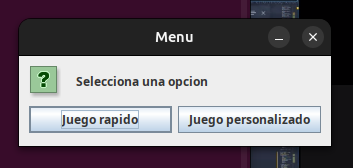
\includegraphics[width=10cm]{latex/img/1.png}
\end{center}

            
\item Estamos a punto de crear un juego personalizado, donde seleccionaremos a los pueblos de Macondo y Rivendel para participar.
\begin{center}
    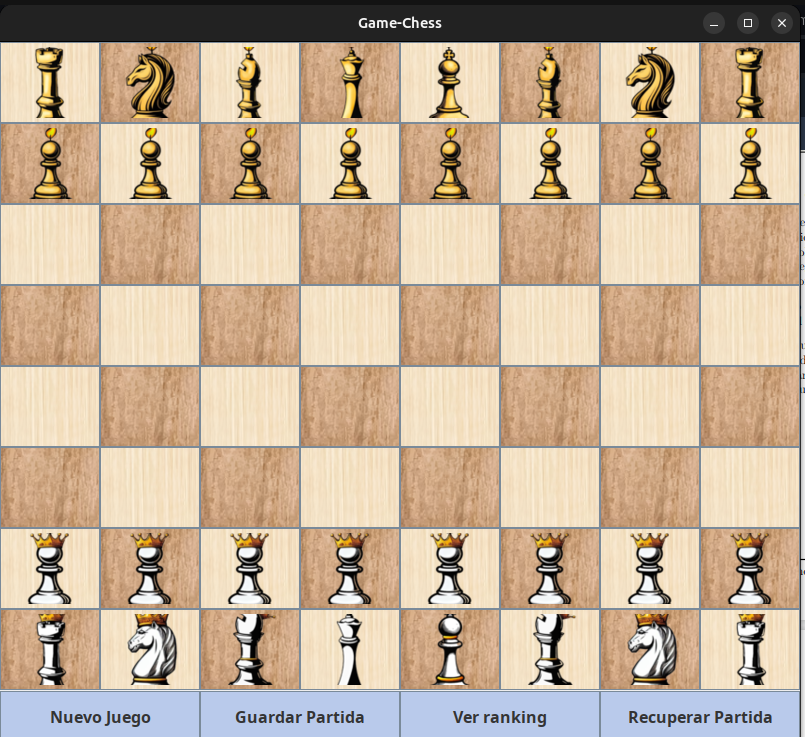
\includegraphics[width=16cm]{latex/img/2.png}
\end{center}

\item La ejecución del juego ha comenzado, y nos encontramos en un tablero con una disposición similar al de un tablero de ajedrez. Ahora exploraremos las opciones disponibles, las cuales incluyen la capacidad de guardar la partida para su recuperación posterior, acceder al ranking de jugadores y comenzar un nuevo juego.
\begin{center}
    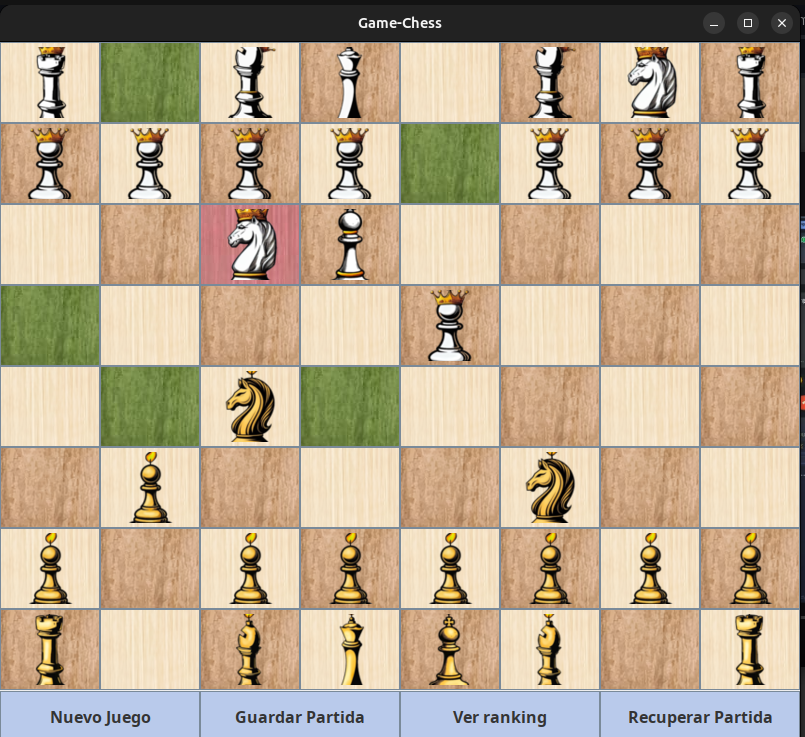
\includegraphics[width=16cm]{latex/img/3.png}
\end{center}

\item El juego se desarrolla por turnos, y al realizar un movimiento, las casillas se pintan de rojo o verde según su disponibilidad para el próximo movimiento. Las casillas rojas indican que no están disponibles, mientras que las casillas verdes señalan opciones válidas para realizar el movimiento en el turno actual. Este sistema de visualización facilita al jugador la toma de decisiones estratégicas durante el juego.
\begin{center}
    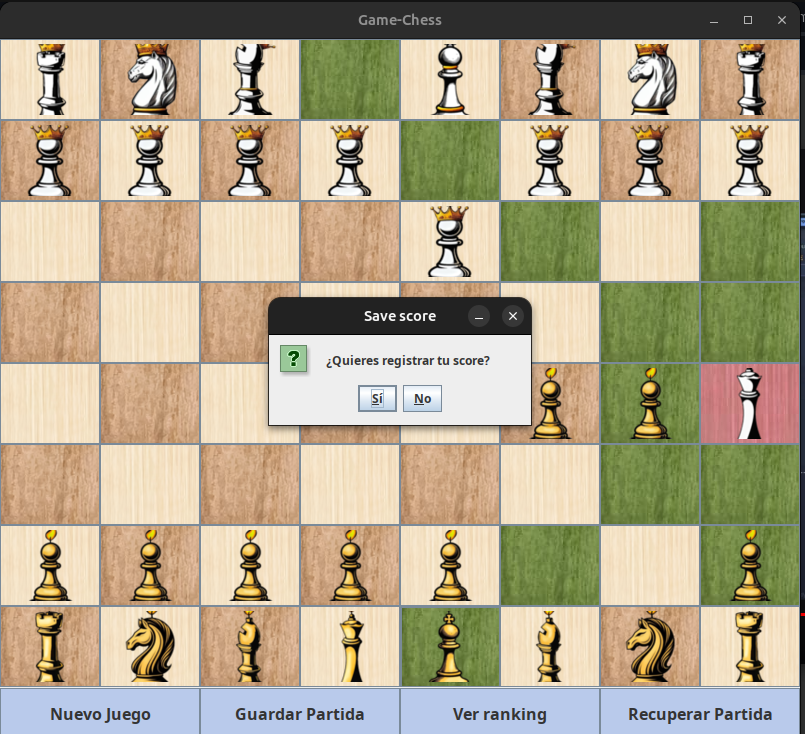
\includegraphics[width=16cm]{latex/img/4.png}
\end{center}



\item En el ámbito de la base de datos, hemos implementado un sistema de récords que registra las partidas ganadas con el menor número posible de jugadas. Al concluir una partida, se presenta una ventana que permite al jugador guardar su puntuación. Para realizar esta acción, el jugador debe ingresar su nombre y, al hacer clic en "Guardar", la información se registra en la base de datos. Posteriormente, se muestra nuevamente la ventana principal, brindando la opción de iniciar un nuevo juego. 
\begin{center}
    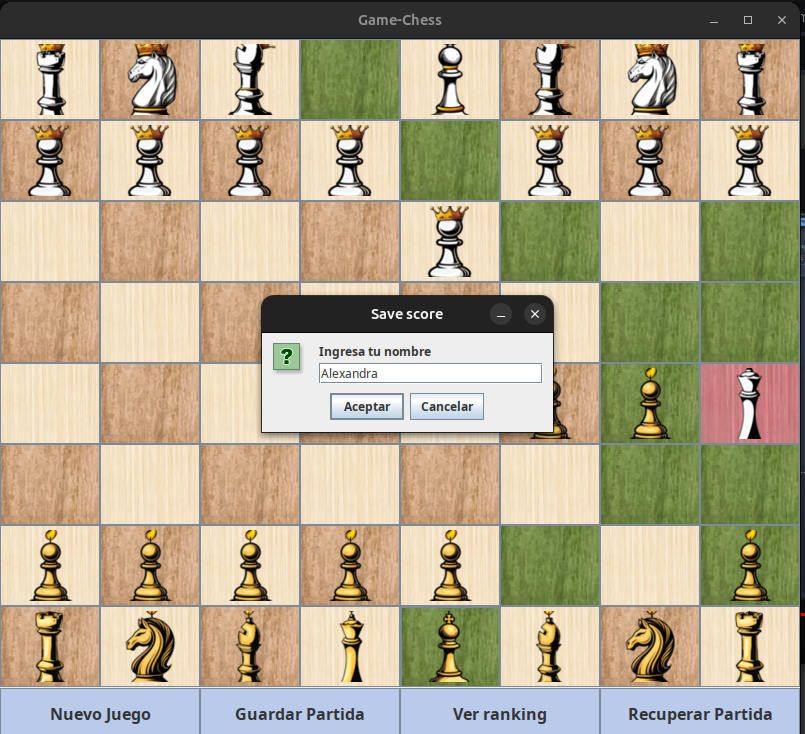
\includegraphics[width=16cm]{latex/img/5.png}
\end{center}


\item En caso de que la instancia del juego se corte, aún se puede acceder a los rankings mediante el botón "Ver Ranking". Este botón realiza una consulta a la base de datos, mostrando así las puntuaciones registradas, incluyendo el último registro efectuado, como el jaque mate con 5 jugadas que acabamos de realizar . Esta función garantiza que los récords y las estadísticas de juego estén siempre disponibles para su visualización.
\begin{center}
    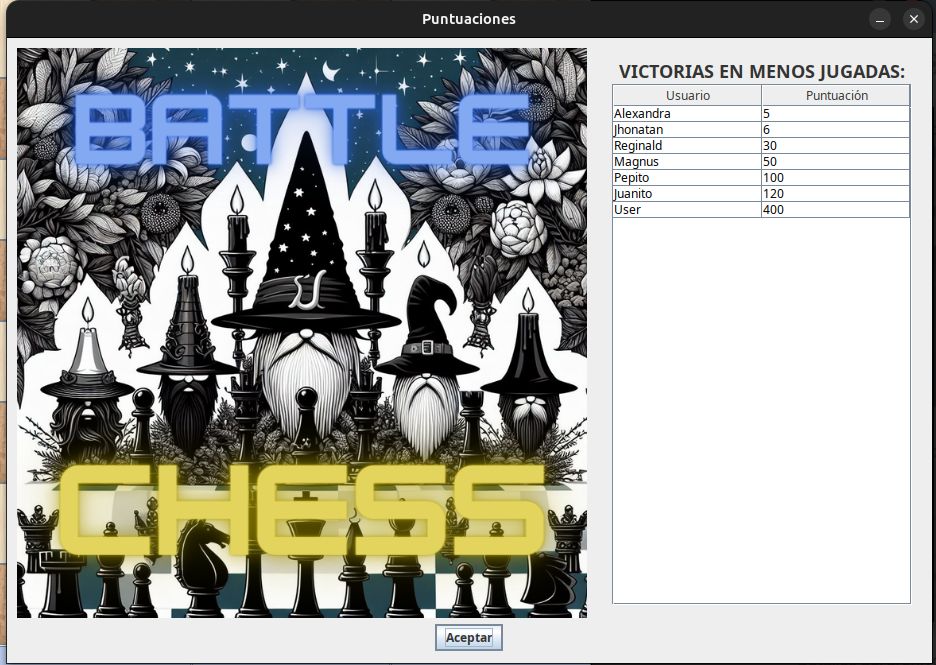
\includegraphics[width=16cm]{latex/img/6.png}
\end{center}



   \end{itemize}





%%%%%%%%%%%%%%%%%%%%%%%%%%%%%%%%%%%%%%%%%%%%%%%%%%%%%%%%%%%%%%%%%%%%%%%%%%%%%%%%%%%%%%%%%%%%%%%%%%%%%%%%%%%%%%%%%%%%%%%%%%%%%%%%%%%%%%%%%%%%%%%%%%%%%%%%%%%%%%%%%%%%%%%%%%%%%%%%%%%%%%%%%%%%%%%%%%%
	\section{\textcolor{red}{Rúbricas}}
	
	\subsection{\textcolor{red}{Entregable Informe}}
	\begin{table}[H]
		\caption{Tipo de Informe}
		\setlength{\tabcolsep}{0.5em} % for the horizontal padding
		{\renewcommand{\arraystretch}{1.5}% for the vertical padding
		\begin{tabular}{|p{3cm}|p{12cm}|}
			\hline
			\multicolumn{2}{|c|}{\textbf{\textcolor{red}{Informe}}}  \\
			\hline 
			\textbf{\textcolor{red}{Latex}} & \textcolor{blue}{El informe está en formato PDF desde Latex,  con un formato limpio (buena presentación) y facil de leer.}   \\ 
			\hline 
			
			
		\end{tabular}
	}
	\end{table}



	\subsection{\textcolor{red}{Rúbrica para el contenido del Informe y demostración}}
	\begin{itemize}			
		\item El alumno debe marcar o dejar en blanco en celdas de la columna \textbf{Checklist} si cumplio con el ítem correspondiente.
		\item Si un alumno supera la fecha de entrega,  su calificación será sobre la nota mínima aprobada, siempre y cuando cumpla con todos lo items.
		\item El alumno debe autocalificarse en la columna \textbf{Estudiante} de acuerdo a la siguiente tabla:
	
		\begin{table}[ht]
			\caption{Niveles de desempeño}
			\begin{center}
			\begin{tabular}{ccccc}
    			\hline
    			 & \multicolumn{4}{c}{Nivel}\\
    			\cline{1-5}
    			\textbf{Puntos} & Insatisfactorio 25\%& En Proceso 50\% & Satisfactorio 75\% & Sobresaliente 100\%\\
    			\textbf{2.0}&0.5&1.0&1.5&2.0\\
    			\textbf{4.0}&1.0&2.0&3.0&4.0\\
    		\hline
			\end{tabular}
		\end{center}
	\end{table}	
	
	\end{itemize}
	
	\begin{table}[H]
		\caption{Rúbrica para contenido del Informe y demostración}
		\setlength{\tabcolsep}{0.5em} % for the horizontal padding
		{\renewcommand{\arraystretch}{1.5}% for the vertical padding
		%\begin{center}
		\begin{tabular}{|p{2.7cm}|p{7cm}|x{1.3cm}|p{1.2cm}|p{1.5cm}|p{1.1cm}|}
			\hline
    		\multicolumn{2}{|c|}{Contenido y demostración} & Puntos & Checklist & Estudiante & Profesor\\
			\hline
			\textbf{1. GitHub} & Hay enlace URL activo del directorio para el  laboratorio hacia su repositorio GitHub con código fuente terminado y fácil de revisar. &2 &X &2 & \\ 
			\hline
			\textbf{2. Commits} &  Hay capturas de pantalla de los commits más importantes con sus explicaciones detalladas. (El profesor puede preguntar para refrendar calificación). &4 &X &3 & \\ 
			\hline 
			\textbf{3. Código fuente} &  Hay porciones de código fuente importantes con numeración y explicaciones detalladas de sus funciones. &2 &X &2 & \\ 
			\hline 
			\textbf{4. Ejecución} & Se incluyen ejecuciones/pruebas del código fuente  explicadas gradualmente. &2 &X &1 & \\ 
			\hline			
			\textbf{5. Pregunta} & Se responde con completitud a la pregunta formulada en la tarea.  (El profesor puede preguntar para refrendar calificación).  &2 &X &1 & \\ 
			\hline	
			\textbf{6. Fechas} & Las fechas de modificación del código fuente estan dentro de los plazos de fecha de entrega establecidos. &2 &X &2 & \\ 
			\hline 
			\textbf{7. Ortografía} & El documento no muestra errores ortográficos. &2 &X &2 & \\ 
			\hline 
			\textbf{8. Madurez} & El Informe muestra de manera general una evolución de la madurez del código fuente,  explicaciones puntuales pero precisas y un acabado impecable.   (El profesor puede preguntar para refrendar calificación).  &4 &X &3 & \\ 
			\hline
			\multicolumn{2}{|c|}{\textbf{Total}} &20 & &19 & \\ 
			\hline
		\end{tabular}
		%\end{center}
		%\label{tab:multicol}
		}
	\end{table}
	
\clearpage

\section{Referencias}
\begin{itemize}			
	\item \url{https://www.geeksforgeeks.org/insertion-sort/}
\end{itemize}	
	
%\clearpage
%\bibliographystyle{apalike}
%\bibliographystyle{IEEEtranN}
%\bibliography{bibliography}
			
\end{document}
